%%%%%%%%%%%%%%%%%%%%%%%%%%%%%%%%%%%%%%%%%%%%%%%%%%%%%%%%
% Tech GreenHouse Node
% Copyright (C) 2016 Marco Giammarini
%
% Author(s):
%  Marco Giammarini <m.giammarini@warcomeb.it>
%
% This program is free software: you can redistribute it and/or modify
% it under the terms of the GNU General Public License as published by
% the Free Software Foundation, either version 3 of the License, or
% any later version.
%
% This program is distributed in the hope that it will be useful,
% but WITHOUT ANY WARRANTY; without even the implied warranty of
% MERCHANTABILITY or FITNESS FOR A PARTICULAR PURPOSE.  See the
% GNU General Public License for more details.
%
% You should have received a copy of the GNU General Public License
% along with this program. If not, see <http://www.gnu.org/licenses/>
%
% The compiled version of this file is licensed under the:
% Creative Commons Attribution-ShareAlike 4.0 International License
% To view a copy of the license, visit <http://creativecommons.org/licenses/by-sa/4.0
%%%%%%%%%%%%%%%%%%%%%%%%%%%%%%%%%%%%%%%%%%%%%%%%%%%%%%%
 
 \documentclass{standalone}

\usepackage{tikz}
\newcommand{\mylsize}[1]{\small{\textbf{#1}}} 
\newcommand{\mysize}[1]{\footnotesize{\textbf{#1}}} 
\newcommand{\myssize}[1]{\tiny{\textbf{#1}}} 

\usetikzlibrary{calc}

%%%%%%%%%%%%%%%%%%%%%%%%%%%%%%%%%%%%%%%%%%%%%%%%%%%%%%%
% Metadata for block definitions
%%%%%%%%%%%%%%%%%%%%%%%%%%%%%%%%%%%%%%%%%%%%%%%%%%%%%%%
\def\tableblockcenter{2}
\def\tableblockwdth{4}

%\def\frdmnum{4}
%\def\frdmheight{\frdmnum * 0.5 +1.5}
\def\frdmheight{3}

\def\supplyheight{3}

\def\stmheight{2}

\begin{document}

\begin{tikzpicture}

%\draw[help lines, style=gray] (0,0) grid (25,25);

% FRDM
\node (frdm) at (10,10){};
\draw [fill=orange, fill opacity=.2] (frdm) rectangle ($(frdm)+(\tableblockwdth , \frdmheight)$);
\node at ($(frdm)+(\tableblockcenter , \frdmheight/2)$) {\mysize{FRDM-KL25Z}};

% SUPPLY
\node (supply) at (16,10){};
\draw  (supply) rectangle ($(supply)+(\tableblockwdth , \supplyheight)$);
\draw  ($(supply)+(\tableblockwdth/2  , 0)$)--($(supply)+(\tableblockwdth/2 , \supplyheight)$);
\node at ($(supply)+(1 , \supplyheight/2 - + \supplyheight/4)$) {\mysize{3V3}};
\draw[thin]($(supply)+(0  , \supplyheight/2)$)--($(supply)+(\tableblockwdth/2 ,\supplyheight/2)$);
\node at ($(supply)+(1 , \supplyheight/2 + \supplyheight/4)$) {\mysize{5V}};
\node at ($(supply)+(\tableblockwdth/2 + 1 , \supplyheight/2)$) {\mylsize{12V}};

% STM
\node (stm) at (16,14){};
\draw (stm) rectangle ($(stm)+(\tableblockwdth , \stmheight)$);
\node at ($(stm)+(\tableblockcenter , \stmheight/2)$) {\mysize{STM WiFi}};

%% EXTERNAL COMPONENT
\draw[dotted](0,9)--(21,9);

% MOISTURE 1
\node (moi1) at (16,6){};
\node [above right, inner sep=0pt, outer sep=0pt] at (moi1) {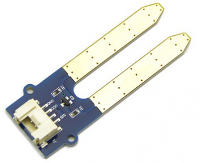
\includegraphics[width=2cm]{images/moisture}};
\draw (moi1) rectangle ($(moi1)+(2 , 2)$);

% MOISTURE 2
\node (moi2) at (19,6){};
\node [above right, inner sep=0pt, outer sep=0pt] at (moi2) {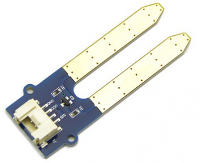
\includegraphics[width=2cm]{images/moisture}};
\draw (moi2) rectangle ($(moi2)+(2 , 2)$);

% MOISTURE 3
\node (moi3) at (16,3){};
\node [above right, inner sep=0pt, outer sep=0pt] at (moi3) {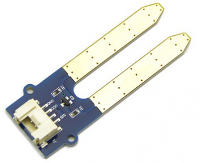
\includegraphics[width=2cm]{images/moisture}};
\draw (moi3) rectangle ($(moi3)+(2 , 2)$);

% MOISTURE 4
\node (moi4) at (19,3){};
\node [above right, inner sep=0pt, outer sep=0pt] at (moi4) {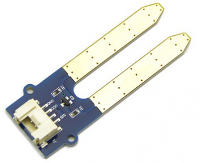
\includegraphics[width=2cm]{images/moisture}};
\draw (moi4) rectangle ($(moi4)+(2 , 2)$);

%%%%%%%%%%%%%%%%%%%%%%%%%%%%%%%%%%% LINE
% POWER SUPPLY INPUT
\draw[<-,ultra thick]($(supply)+( \tableblockwdth , \supplyheight/2)$)--($(supply)+ ( \tableblockwdth + 1, \supplyheight/2)$);


\end{tikzpicture}
\end{document}